

\documentclass[12p]{article}
\usepackage[english]{babel}
\usepackage{microtype}   
\usepackage[left=3cm, right=3cm]{geometry}		                                % Margins left and right
\usepackage{hyperref}                                                           % Clickable table of contents in PDFs
\usepackage{datetime}                                                           % Currenttime
\usepackage{graphicx}                                                           % Import .pdf-files as figure
\usepackage{subcaption}                                                         % Subfigure
\usepackage{float}                                                              % float [H]

\usepackage{physics}                                                            % Physics typesetting: bra-ket
\usepackage{amsfonts}                                                           % mathfrak
\usepackage{mathtools}                                                          % dcases, DeclarePairedDelimiter
\usepackage{amsmath}


\title{CI: Computational Details}
\author{Tobias Huysentruyt \\ GQCG}

\begin{document}

\maketitle

% % % ABSTRACT AND TABLE OF CONTENTS

% Abstract
\begin{abstract} \noindent  % enters inside the abstract are not rendered as line breaks in the .pdf-file
    These notes serve as a supplementary tool to understand the GQCP code, or write your own CI codes
\end{abstract}

% Line after abstract
\begin{center}
    \line(1,0){250}
\end{center}

% Table of contents
\tableofcontents
\newpage

% % % MAIN TEXT % % %

\newpage

\section{Two-Electron Off-Diagonal Address Calculation}


\subsection{Calculating Addresses}
Calculating the address of an ONV can be done via the addressing scheme of the Fock space.
(REF Lemmens 8.4.3 An addressing scheme for spin strings) \\
This is particullary important for DOCI where one cannot store sub calculations of the Hamiltonian, and the performance of the matvec will greatly be impacted by how fast you can generate the Hamiltonian (while in FCI one can perform the matvec with significantly smaller sparse matrixes).
\subsubsection{One electron operators}
Take the following calculation on an ONV with address 5 (starting from 0) in a K=5 N=3 Fock space: \\
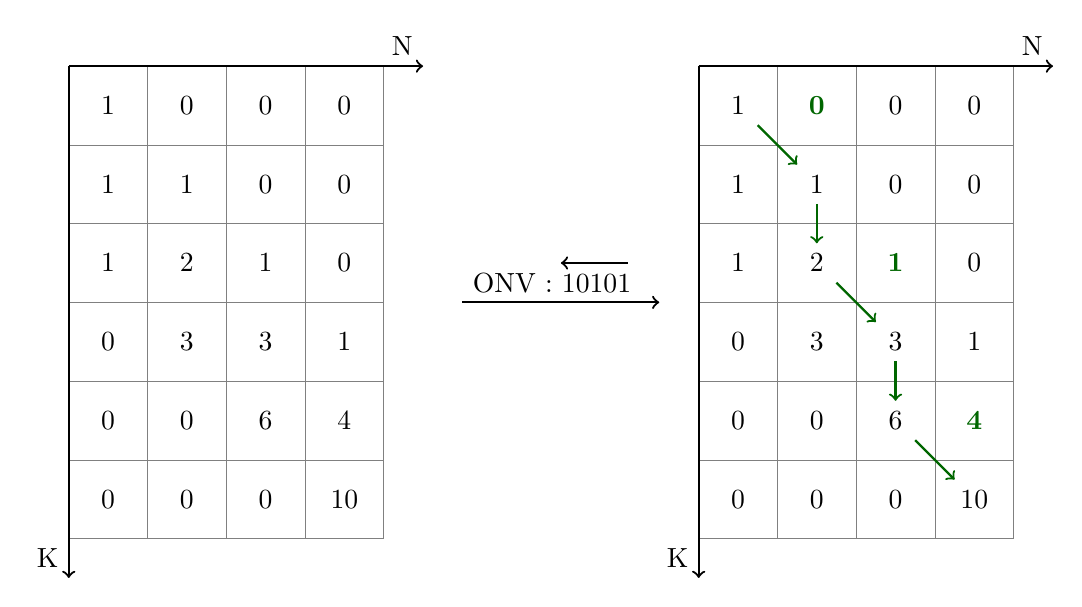
\begin{tikzpicture}
\draw[step=1cm,gray,very thin] (-2,-2) grid (2,4);
\draw[thick,->] (-2,4) -- (2.5,4) node[anchor=south east] {N};
\draw[thick,->] (-2,4) -- (-2,-2.5) node[anchor=south east] {K};

\node at (-1.5,3.5) {1};
\node at (-1.5,2.5) {1};
\node at (-1.5,1.5) {1};
\node at (-1.5,0.5) {0};
\node at (-1.5,-0.5) {0};
\node at (-1.5,-1.5) {0};

\node at (-0.5,3.5) {0};
\node at (-0.5,2.5) {1};
\node at (-0.5,1.5) {2};
\node at (-0.5,0.5) {3};
\node at (-0.5,-0.5) {0};
\node at (-0.5,-1.5) {0};

\node at (0.5,3.5) {0};
\node at (0.5,2.5) {0};
\node at (0.5,1.5) {1};
\node at (0.5,0.5) {3};
\node at (0.5,-0.5) {6};
\node at (0.5,-1.5) {0};

\node at (1.5,3.5) {0};
\node at (1.5,2.5) {0};
\node at (1.5,1.5) {0};
\node at (1.5,0.5) {1};
\node at (1.5,-0.5) {4};
\node at (1.5,-1.5) {10};

\draw[thick,<-] (5.5,1) -- (3,1) node[anchor=south west] {ONV : 10101};
\draw[thick,->] (5.10,1.5) -- (4.25,1.5);
\draw[step=1cm,gray,very thin] (6,-2) grid (10,4);

\draw[thick,->] (6,4) -- (10.5,4) node[anchor=south east] {N};
\draw[thick,->] (6,4) -- (6,-2.5) node[anchor=south east] {K};

\node at (6.5,3.5) {1};
\node at (6.5,2.5) {1};
\node at (6.5,1.5) {1};
\node at (6.5,0.5) {0};
\node at (6.5,-0.5) {0};
\node at (6.5,-1.5) {0};

\node at (7.5,3.5) {\textbf{\textcolor{black!60!green}{0}}};
\node at (7.5,2.5) {1};
\node at (7.5,1.5) {2};
\node at (7.5,0.5) {3};
\node at (7.5,-0.5) {0};
\node at (7.5,-1.5) {0};

\node at (8.5,3.5) {0};
\node at (8.5,2.5) {0};
\node at (8.5,1.5) {\textbf{\textcolor{black!60!green}{1}}};
\node at (8.5,0.5) {3};
\node at (8.5,-0.5) {6};
\node at (8.5,-1.5) {0};

\node at (9.5,3.5) {0};
\node at (9.5,2.5) {0};
\node at (9.5,1.5) {0};
\node at (9.5,0.5) {1};
\node at (9.5,-0.5) {\textbf{\textcolor{black!60!green}{4}}};
\node at (9.5,-1.5) {10};

\draw[thick, black!60!green, ->] (6.75,3.25) -- (7.25,2.75);
\draw[thick, black!60!green, ->] (7.50,2.25) -- (7.50,1.75);
\draw[thick, black!60!green, ->] (7.75,1.25) -- (8.25,0.75);
\draw[thick, black!60!green, ->] (8.50,0.25) -- (8.50,-0.25);
\draw[thick, black!60!green, ->] (8.75,-0.75) -- (9.25,-1.25);
\end{tikzpicture}
\\
After performing an annihilation on electron position zero, and creating an electron on position 3 we arrivate at:
\\
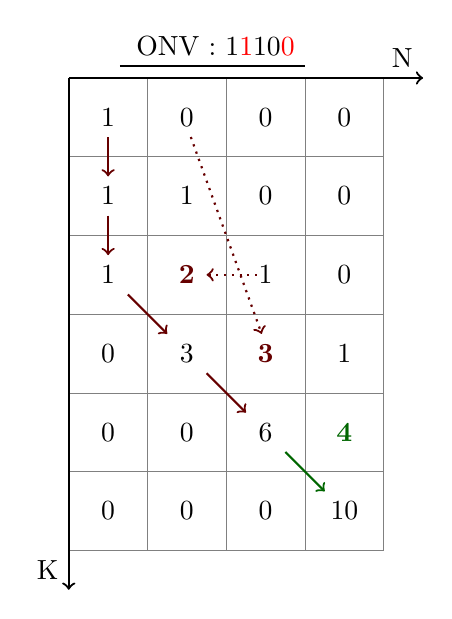
\begin{tikzpicture}
\draw[thick,-] (-1.35,4.15) -- (1,4.15) node[anchor=south east] {ONV : 1\textcolor{red}{1}10\textcolor{red}{0}};
\draw[step=1cm,gray,very thin] (-2,-2) grid (2,4);
\draw[thick,->] (-2,4) -- (2.5,4) node[anchor=south east] {N};
\draw[thick,->] (-2,4) -- (-2,-2.5) node[anchor=south east] {K};

\node at (-1.5,3.5) {1};
\node at (-1.5,2.5) {1};
\node at (-1.5,1.5) {1};
\node at (-1.5,0.5) {0};
\node at (-1.5,-0.5) {0};
\node at (-1.5,-1.5) {0};

\node at (-0.5,3.5) {0};
\node at (-0.5,2.5) {1};
\node at (-0.5,1.5) {\textbf{\textcolor{black!60!red}{2}}};
\node at (-0.5,0.5) {3};
\node at (-0.5,-0.5) {0};
\node at (-0.5,-1.5) {0};

\node at (0.5,3.5) {0};
\node at (0.5,2.5) {0};
\node at (0.5,1.5) {1};
\node at (0.5,0.5) {\textbf{\textcolor{black!60!red}{3}}};
\node at (0.5,-0.5) {6};
\node at (0.5,-1.5) {0};

\node at (1.5,3.5) {0};
\node at (1.5,2.5) {0};
\node at (1.5,1.5) {0};
\node at (1.5,0.5) {1};
\node at (1.5,-0.5) {\textbf{\textcolor{black!60!green}{4}}};
\node at (1.5,-1.5) {10};

\draw[thick, black!60!red, ->] (-1.5,3.25) -- (-1.5,2.75);
\draw[thick, black!60!red, ->] (-1.5,2.25) -- (-1.5,1.75);
\draw[thick, black!60!red, ->] (-1.25,1.25) -- (-0.75,0.75);
\draw[thick, black!60!red, ->] (-0.25,0.25) -- (0.25,-0.25);
\draw[thick, black!60!green, ->] (0.75,-0.75) -- (1.25,-1.25);

\draw[thick, dotted, black!60!red, ->] (-0.45,3.25) -- (0.45,0.75);
\draw[thick, dotted, black!60!red, <-] (-0.25,1.5) -- (0.40,1.5);

\end{tikzpicture}
Only the path in-between the annihilation-creation couple is altered, hence we can calculate the new address from the old address.
Subtract the weight of annihilated and add the weight of the created. Followed by subtracting the old weight of the altered path by that of the new weight to update the address. As an example, our initial address was 5, annihilated weight from electron one, on position zero: $W_{0,1}$, weight from the created electron (now electron two), on position three: $W_{3,2}$. The initial electron two was shifted to electron one (on position two): $W_{2,1} - W_{2,2}$ or $W_{3,2} - 2*W_{2,2}$. This equates to $I - W_{0,1} + W_{3,2} - W_{2,2} + W_{2,1} = J \iff 5 - 0 + 3 - 1 + 2 = 9$
\\
Below is an other example:
\\
%
%
%
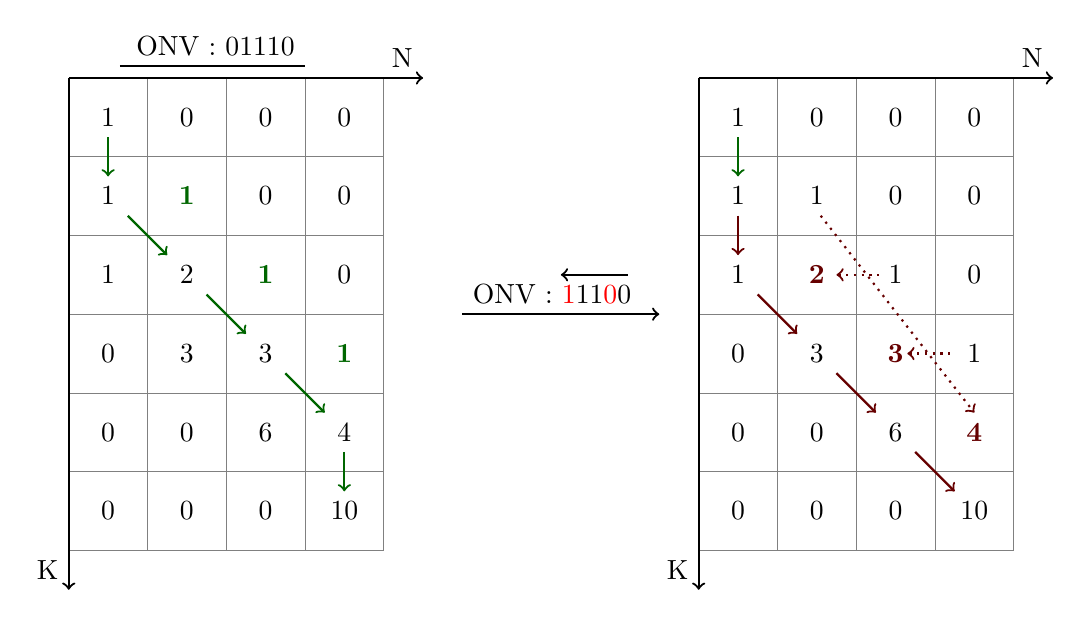
\begin{tikzpicture}
  \draw[thick,-] (-1.35,4.15) -- (1,4.15) node[anchor=south east] {ONV : 01110};
  \draw[step=1cm,gray,very thin] (-2,-2) grid (2,4);
  \draw[thick,->] (-2,4) -- (2.5,4) node[anchor=south east] {N};
  \draw[thick,->] (-2,4) -- (-2,-2.5) node[anchor=south east] {K};


  \node at (-1.5,3.5) {1};
  \node at (-1.5,2.5) {1};
  \node at (-1.5,1.5) {1};
  \node at (-1.5,0.5) {0};
  \node at (-1.5,-0.5) {0};
  \node at (-1.5,-1.5) {0};

  \node at (-0.5,3.5) {0};
  \node at (-0.5,2.5) {\textbf{\textcolor{black!60!green}{1}}};
  \node at (-0.5,1.5) {2};
  \node at (-0.5,0.5) {3};
  \node at (-0.5,-0.5) {0};
  \node at (-0.5,-1.5) {0};

  \node at (0.5,3.5) {0};
  \node at (0.5,2.5) {0};
  \node at (0.5,1.5) {\textbf{\textcolor{black!60!green}{1}}};
  \node at (0.5,0.5) {3};
  \node at (0.5,-0.5) {6};
  \node at (0.5,-1.5) {0};

  \node at (1.5,3.5) {0};
  \node at (1.5,2.5) {0};
  \node at (1.5,1.5) {0};
  \node at (1.5,0.5) {\textbf{\textcolor{black!60!green}{1}}};
  \node at (1.5,-0.5) {4};
  \node at (1.5,-1.5) {10};

  \draw[thick, black!60!green, ->] (-1.50,3.25) -- (-1.50,2.75);
  \draw[thick, black!60!green, ->] (-1.25,2.25) -- (-0.75,1.75);
  \draw[thick, black!60!green, ->] (-0.25,1.25) -- (0.25,0.75);
  \draw[thick, black!60!green, ->] (0.75,0.25) -- (1.25,-0.25);
  \draw[thick, black!60!green, ->] (1.50,-0.75) -- (1.50,-1.25);

\draw[thick,<-] (5.5,1) -- (3,1) node[anchor=south west] {ONV : \textcolor{red}{1}11\textcolor{red}{0}0};
\draw[thick,->] (5.10,1.5) -- (4.25,1.5);
\draw[step=1cm,gray,very thin] (6,-2) grid (10,4);

\draw[thick,->] (6,4) -- (10.5,4) node[anchor=south east] {N};
\draw[thick,->] (6,4) -- (6,-2.5) node[anchor=south east] {K};

\node at (6.5,3.5) {1};
\node at (6.5,2.5) {1};
\node at (6.5,1.5) {1};
\node at (6.5,0.5) {0};
\node at (6.5,-0.5) {0};
\node at (6.5,-1.5) {0};

\node at (7.5,3.5) {0};
\node at (7.5,2.5) {1};
\node at (7.5,1.5) {\textbf{\textcolor{black!60!red}{2}}};
\node at (7.5,0.5) {3};
\node at (7.5,-0.5) {0};
\node at (7.5,-1.5) {0};

\node at (8.5,3.5) {0};
\node at (8.5,2.5) {0};
\node at (8.5,1.5) {1};
\node at (8.5,0.5) {\textbf{\textcolor{black!60!red}{3}}};
\node at (8.5,-0.5) {6};
\node at (8.5,-1.5) {0};

\node at (9.5,3.5) {0};
\node at (9.5,2.5) {0};
\node at (9.5,1.5) {0};
\node at (9.5,0.5) {1};
\node at (9.5,-0.5) {\textbf{\textcolor{black!60!red}{4}}};
\node at (9.5,-1.5) {10};

\draw[thick, black!60!green, ->] (6.50,3.25) -- (6.50,2.75);
\draw[thick, black!60!red, ->] (6.50,2.25) -- (6.50,1.75);
\draw[thick, black!60!red, ->] (6.75,1.25) -- (7.25,0.75);
\draw[thick, black!60!red, ->] (7.75,0.25) -- (8.25,-0.25);
\draw[thick, black!60!red, ->] (8.75,-0.75) -- (9.25,-1.25);

\draw[thick, dotted, black!60!red, ->] (7.55,2.25) -- (9.50,-0.25);
\draw[thick, dotted, black!60!red, <-] (8.65,0.5) -- (9.25,0.5);
\draw[thick, dotted, black!60!red, <-] (7.75,1.5) -- (8.35,1.5);
\end{tikzpicture}
\\
In this case two adjacent electrons are shifted. The total shift of multiple shifted electrons can be calculated simultaneously:
\begin{equation}
  \sum^{l}_{i = 0} (W_{k +i,n-1 +i} - W_{k+i,n+i}) = W_{k+1+l, n-1+l} - W_{k+1+l,n+l} - W_{k, n-2} + W_{k,n-1}
\end{equation}
starting from $W_{2,2}$ in the above example for two electrons $(i \in [0,1])$:
\begin{equation}
W_{4, 2} - W_{4,3} - W_{2, 0} + W_{2,1} =  6-4 - 1 + 2 = 3
\end{equation}
With an initial address of 3, a creation-annhilation shift of 3 and a path shift of 3, we find $3+3+3 = 9$

It is often beneficial to generate all one-electron coupling sequentially so that your algorithm progresses sequentially through memory rather than discontionious or seemingly random. \\

\begin{algorithm}[H]\label{al:one-op}
 \KwResult{Generate all upper diagonal one-electron Hamiltonian elements}
 \For{ONV in Fock space}{
  \For{Occupied electron positions}{
  \textbf{Set} address and update according to annihilation \\
  \If{next occupied position - initial position $>$ 1} {
    \textbf{update} address through \textbf{shift} \\
    $sign = -1^{next occupied position - initial position - 1}$
  }
  \While{unoccupied positions left}{
      Calculate \textbf{new} address according to creation and calculate the Hamiltonian/RDM element according to the sign and the creation and annhilation indexes \\
      \If{next occupied position - initial position $>$ 1} {
        \textbf{update} address through \textbf{shift} \\
        $sign = sign * -1^{next occupied position - initial position - 1}$
      }
   }
  }
 }
 \caption{Possible one-electron operator algorithm}
\end{algorithm}

The initial total operator sign will always be 1, because if no shift has occured over occupied electrons the creation operator will have the same sign as the annihilation operator making the total sign positive (-1*-1 = 1 or 1*1 = 1).

\subsubsection{Two electron operators}

For DOCI the only non-vanishing off-diagonal coupling operator combinations are two-electron operators which will affect both alpha in beta in the same way such that they can be consdensed to one-electron operators in one Fock space. One can then perform algorithm (\ref{al:one-op}) but without the operator sign (it's always positive). Implementing these efficiently is very important for the DOCI matvec algoritm as its scaling will soley depend on how quickly you can generate all Hamiltonian elements (when one cannot store the Hamiltonian in a sparse matrix)

For FCI, the two-electron algorithm will be a combination of next-shift and back-shift calculations. And which operator combinations are minimal will be discussed in the following section. However, performance of the matvec will not be affected. Because the Hamiltonian elements can be stored sparsely virtually always (see later). The couplings and elements will have to be cacluated once, before the matvec, and will affect performance if it is written so poorly that it requires more execution time than a matvec, or than multiple matvec calls durning the Davidson algorithm.


\newpage

\section{Hamiltonian Elements}

Given a Fock space.
\\
Let us call $\ket{I_{\alpha}}$ the ONV with address I.
We have arrived at following expression for the Hamiltonian (ref lemmens):

      \begin{equation}\label{eq:ham}
          \hat{\mathcal{H}}_\text{elec} = \sum_{pq}^K k_{pq} \hat{E}_{pq} + \frac{1}{2} \sum_{pqrs}^K g_{pqrs} \hat{E}_{pq} \hat{E}_{rs}
      \end{equation}
We will focus only on the two electron operators $ \sum_{pqrs}^K g_{pqrs} \hat{a}^{\dagger}_{p} \hat{a}_{q}  \hat{a}^{\dagger}_{r} \hat{a}_{s}$. And only focus on the $\alpha$ electrons. We will therefore ignore the $\alpha$ subscript.
We require to consider operator indices for which a given ONV I does not vanish:
\begin{equation} \label{eq:address}
  \bra{I} \hat{a}^{\dagger}_{p} \hat{a}_{q} \hat{a}^{\dagger}_{r} \hat{a}_{s} = \bra{J}
\end{equation}
In which $J$ is an address larger than $I$. Reason for this is, in the event that $\ket{I}$ can be transformed in $\ket{J}$. $\ket{J}$ can also be transformed back to $\ket{I}$ yielding the same two-electron term (hermitian two-electron operators).

\begin{equation}
  (\bra{I} E_{pq} E_{rs} \ket{J})^\dagger = \bra{J} E_{sr} E_{qp} \ket{I}
\end{equation}

It is important to note, that I will base further explanations from the perspective of equation (\ref{eq:address}) where $\hat{a}^{\dagger}_{p}$ annihilates on $\bra{I}$.

\subsubsection{Minimal operator iterations}
For the address to be larger at all times, the highest index of a creation should always be higher than the highest index of an annihilation. This is easily verified by the fact that we represent our ONVs in binary and that the addressing is based on the ordering of its integer value. Given the relation of numeric value for each index of an integer represented in binary is quadratic, the integer value of a set index is always larger than any combination of previously set indices:
\begin{equation}
  2^N - 1 = \sum^{N-1}_{i=0} 2^i
\end{equation}
Additionally we can state that the first annihiltion can always have a smaller index than the second annihiltion without skipping over any address, the same is true for the creation operators.

Regardless in which way they are executed (if they are all different indices), the address will be the same. However the order of execution can alter the expression (sign wise) and will be accompanied by a different two-electron term. Given an ONV $\bra{I}$ for which $\bra{I} \hat{a}^\dagger_p \hat{a}_q \hat{a}^\dagger_r \hat{a}_s \neq 0 $ we find that:
\begin{align}
  \bra{I} \hat{a}^\dagger_p \hat{a}_q \hat{a}^\dagger_r \hat{a}_s & = \bra{I} (\hat{a}^\dagger_p \hat{a}_s \delta_{rq} - \hat{a}^\dagger_p \hat{a}^\dagger_r \hat{a}_q \hat{a}_s) \nonumber \\
  & = \bra{I} (\hat{a}^\dagger_p  \hat{a}_s \delta_{rq} + \hat{a}^\dagger_r \hat{a}^\dagger_p \hat{a}_q \hat{a}_s) \nonumber \\
  & = \bra{I} (\hat{a}^\dagger_p  \hat{a}_s \delta_{rq} + \hat{a}^\dagger_r \hat{a}_s \delta_{pq} - \hat{a}^\dagger_r \hat{a}_q \hat{a}^\dagger_p \hat{a}_s) \label{eq:equals} \\
  & \text{IF p,q,r,s $\neq$} \nonumber \\
  & = - \bra{I}(\hat{a}^\dagger_r \hat{a}_q \hat{a}^\dagger_p \hat{a}_s )\\
  & = \bra{I} (\hat{a}^\dagger_r \hat{a}_s \hat{a}^\dagger_p \hat{a}_q ) \\
  & = - \bra{I} (\hat{a}^\dagger_p \hat{a}_s \hat{a}^\dagger_r \hat{a}_q)
\end{align}
So for the \textit{p,q,r,s $\neq$} case, we can enforce : $p<r$, $q<s$ for symmetries and anti-symmetries, and $s > r$ upper diagonal to not generate redundant addresses. This leaves us with limited combinations:

\begin{enumerate}
  \item $p > q$ ($s > r > p$)
  \item $p < q$
  \begin{itemize}
    \item $r > q$ ($s > r$)
    \item $q > r$ ($s > q$)
  \end{itemize}
\end{enumerate}
For inplace annihila-crea- and crea-annihila-tions, the rules are slightly different, because creation annihilation operators with the same index cancel each other out. Therefore the non-annihiltion bound creation index has to be larger than the non-creation bound annihiltion index to produce larger addresses (the rules for one-electron evaluation).

\begin{enumerate}
  \item $p = q$, $s > r$
  \item $q = r$, $s > p$
\end{enumerate}
These have some implication for symmetry and anti-symmetry equations such as equation (\ref{eq:equals}) as $\delta$ is not always zero:


\begin{align}
   \bra{I}  \hat{a}^\dagger_p \hat{a}_q \hat{a}^\dagger_r \hat{a}_s & =   \bra{I} (\hat{a}^\dagger_p \hat{a}_s \delta_{rq} + \hat{a}^\dagger_r  \hat{a}_s \delta_{pq} - \hat{a}^\dagger_r \hat{a}_q \hat{a}^\dagger_p \hat{a}_s) \\
  & =   \bra{I} (\hat{a}^\dagger_p \hat{a}_s \delta_{rq} + \hat{a}^\dagger_r \hat{a}_s \delta_{pq} - \hat{a}^\dagger_r \hat{a}_q  \delta_{sp} - \hat{a}^\dagger_r \hat{a}_s \delta_{pq} + \hat{a}^\dagger_r \hat{a}_s \hat{a}^\dagger_p \hat{a}_q) \\
  & =   \bra{I} (\hat{a}^\dagger_p \hat{a}_q \delta_{rs} + \hat{a}^\dagger_p \hat{a}_s \delta_{qr} - \hat{a}^\dagger_p \hat{a}_s \hat{a}^\dagger_r \hat{a}_q)
\end{align}

\subsubsection{$p = q$} \label{p=q}
For $p = q$ we can also see that for $s = q \iff r = q$ ortherwise we would have a double creation on the same index without an annihilation on that same index, which is a vanishing operation sequence. However this does not alter the address (diagonal contribution) and is ignored in the algorithm. Hence we state that $ s \neq p, q, r $ This simplifies the equations:

\begin{align}
  \bra{I}  \hat{a}^\dagger_p \hat{a}_p \hat{a}^\dagger_r \hat{a}_s & =  \bra{I} (\hat{a}^\dagger_p \hat{a}_s \delta_{rp} + \hat{a}^\dagger_r  \hat{a}_s - \hat{a}^\dagger_r \hat{a}_p \hat{a}^\dagger_p \hat{a}_s) \\
  & =   \bra{I} (\hat{a}^\dagger_p \hat{a}_s \delta_{rp} + \hat{a}^\dagger_r \hat{a}_s \hat{a}^\dagger_p \hat{a}_p) \\
  & =   \bra{I} (\hat{a}^\dagger_p \hat{a}_s \delta_{pr} - \hat{a}^\dagger_p \hat{a}_s \hat{a}^\dagger_r \hat{a}_p)
\end{align}
We can then discriminate between $r = p$ :

\begin{align}
    \bra{I} \hat{a}^\dagger_p \hat{a}_p \hat{a}^\dagger_p \hat{a}_s & =   \bra{I} (\hat{a}^\dagger_p \hat{a}_s + \hat{a}^\dagger_p \hat{a}_s - \hat{a}^\dagger_p \hat{a}_p \hat{a}^\dagger_p \hat{a}_s ) \\
  & =   \bra{I} (\hat{a}^\dagger_p \hat{a}_s + \hat{a}^\dagger_p \hat{a}_s \hat{a}^\dagger_p \hat{a}_p) \label{eq:vanish1} \\
  & =   \bra{I} (\hat{a}^\dagger_p \hat{a}_s - \hat{a}^\dagger_p \hat{a}_s \hat{a}^\dagger_p \hat{a}_p) \label{eq:vanish2}
\end{align}
We see in equation (\ref{eq:vanish1}) and (\ref{eq:vanish2}) that last term annihilates $p$, then operator on index $s$ does strictly not create on index $p$ and index $p$ is annihilated again, thus this term vanishes:

\begin{equation}
 \bra{I}  \hat{a}^\dagger_p \hat{a}_p \hat{a}^\dagger_p \hat{a}_s = \bra{I} \hat{a}^\dagger_p \hat{a}_s
\end{equation}
For $r \neq p$:
\begin{align}
    \bra{I} \hat{a}^\dagger_p \hat{a}_p \hat{a}^\dagger_r \hat{a}_s & =   \bra{I} ( \hat{a}^\dagger_r  \hat{a}_s - \hat{a}^\dagger_r \hat{a}_p \hat{a}^\dagger_p \hat{a}_s ) \nonumber \\
  & =   \bra{I} (\hat{a}^\dagger_r  \hat{a}_s) \label{eq:rneqp}\\
  & =   \bra{I} ( \hat{a}^\dagger_r \hat{a}_s \hat{a}^\dagger_p \hat{a}_p) \\
  & = -   \bra{I} (\hat{a}^\dagger_p \hat{a}_s \hat{a}^\dagger_r \hat{a}_p)
\end{align}
Where se see that for equation (\ref{eq:rneqp}) the second term vanished, as the initial term is assumend non-vanishing.

\subsubsection{$q=r$}
We only cover $p \neq r$ as we assume tha $r$ starts unoccupied as opposed to the previous section (\ref{p=q}).
\begin{align}
  \bra{I} \hat{a}^\dagger_p \hat{a}_r \hat{a}^\dagger_r \hat{a}_s & =   \bra{I} (\hat{a}^\dagger_p \hat{a}_s - \hat{a}^\dagger_r \hat{a}_r \hat{a}^\dagger_p \hat{a}_s) \nonumber \\
  & =   \bra{I} \hat{a}^\dagger_p \hat{a}_s  \\
  & =   \bra{I} (\hat{a}^\dagger_p \hat{a}_s + \hat{a}^\dagger_r \hat{a}_s \delta_{pr} - \hat{a}^\dagger_r \hat{a}_r  \delta_{sp} - \hat{a}^\dagger_r \hat{a}_s \delta_{pr} + \hat{a}^\dagger_r \hat{a}_s \hat{a}^\dagger_p \hat{a}_r) \\
  & =   \bra{I} (\hat{a}^\dagger_p \hat{a}_r \delta_{rs} + \hat{a}^\dagger_p \hat{a}_s - \hat{a}^\dagger_p \hat{a}_s \hat{a}^\dagger_r \hat{a}_r)
\end{align}
Which simplifies to:
\begin{equation}
    \bra{I} \hat{a}^\dagger_p \hat{a}_r \hat{a}^\dagger_r \hat{a}_s =   \bra{I} \hat{a}^\dagger_p \hat{a}_s
\end{equation}


\subsubsection{Summary for the Hamiltonian}
In short this we shall sum up what appears to be the minimal amount of operators required to retrieve all information for the Hamiltonian for the two-electron (same spin) operators.
The value:
\begin{equation}
  \frac{1}{2} (g_{pqrs} + g_{rspq} - g_{rqps} - g_{psrq})
\end{equation}
 Can be retrieved for any of the follwing non-vanishing operator sequence combinations yielding a higher and the same (thus non redundant) address for a given $\bra{I}$:
\begin{enumerate}
  \item $s > r > p > q$
  \item $s > r > q > p$
  \item $s > q > r > p$
\end{enumerate}
For every occupied index $x$ in an ONV:
\begin{equation}
  \frac{1}{2} (g_{xxpq} + g_{pqxx} - g_{xpqx})
\end{equation}
We can also see that for $p=x$ we arrive at:
\begin{equation}
  \frac{1}{2} (g_{xxxq})
\end{equation}
For every unnocupied index $y$ ($p \neq y$) in an ONV:
\begin{equation}
  \frac{1}{2} (g_{pyyq})
\end{equation}
Where for both cases $p<q$.

\section{The FCI (restricted) matrix vector product}

Internally it is recommended to work with relative addresses for both spin functions and then order them logically in your total vectors. Given the nature of our Hamiltonian (total operators do not affect spin) we can write an ONV as two ONVs from two seperate Fock spaces (and have the total Fock space be a direct product of those spaces). $\ket{ONV} = \ket{ONV_\alpha ONV_\beta}$. Choose one of the ONVs to be major and the other minor. If for example your $\alpha$ Fock space is major your $ONV_\alpha$ will permutate after a full permutation of your $ONV_\beta$ which are $\beta$ Fock space dimension permutations.
We define $\textbf{dim}_\alpha$ as the $\alpha$ Fock space dimension and $\textbf{dim}_\beta$ as the $\beta$ Fock space dimension and the total dimension $\textbf{dim}_{total} = \textbf{dim}_\alpha * \textbf{dim}_\beta$. \\
An eigenvector is thus stored as such:
\begin{tabular}{|l|l||l|}
\hline
$I_{\alpha}$ & $I_{\beta}$ & $I_{\textbf{total}}$ \\ \hline
$I_1$ & $I_1$ & $I_1$ \\ \hline
$I_1$ & $I_2$ & $I_2$ \\ \hline
$I_1$ & $I_3$ & $I_3$ \\ \hline
$I_1$ & $I_{...}$ & $I_{...}$ \\ \hline
$I_1$ & $I_{\textbf{dim}_\beta}$ & $I_{\textbf{dim}_\beta}$ \\ \hline
$I_2$ & $I_{1}$ & $I_{\textbf{dim}_\beta + 1}$ \\ \hline
$I_2$ & $I_{2}$ & $I_{\textbf{dim}_\beta + 2}$ \\ \hline
$I_{...}$ & $I_{...}$ & $I_{... * \textbf{dim}_\beta + ...}$ \\ \hline
$I_{\textbf{dim}_\alpha}$ & $I_{\textbf{dim}_\beta}$ & $I_{\textbf{dim}_{total}}$ \\ \hline
\end{tabular}
\\
Rudimentary approach to performing the matrix vector product for a none storable Hamiltonian can be done as follows (where P is the vector resulting from the product and X is the vector partaking in the product):
\begin{align}
  \text{P}_{I} = \sum_J \text{H}_{IJ} * \text{X}_{J} \\
  \text{P}_{J} = \sum_I \text{H}_{JI} * \text{X}_{I}
\end{align}
Where $\text{Hamiltonian}_{JI} = \text{Hamiltonian}_{IJ}$ (or $\text{Hamiltonian}_{JI} = \text{Hamiltonian}_{IJ}^*$ when working complex). Allowing for the upperdiagonal approach (for I coupling to J one finds J coupling to I)

\subsection{Evaluations Seperated by Spin}
For a set of operators only affecting one spin function we can repeat the coupling as many times as there are permutations in the Fock space of the opposite spin. e.g.:
\begin{equation} \label{eq:coupling_alpha}
  \bra{I_\alpha I_\beta} \hat{a}^{\dagger}_{p \alpha} \hat{a}_{q \alpha} \hat{a}^{\dagger}_{r \alpha} \hat{a}_{s \alpha} \ket{J_\alpha I_\beta} \neq 0
\end{equation}
We can calculate a portion of P (all one-electron and part of the two-electron (only the same spin) evaluations), $\text{P}^{\alpha}$ and $\text{P}^{\beta}$.
Where we now define $\text{P} = \text{P}^{\alpha \beta} + \text{P}^{\alpha} + \text{P}^{\beta}$ with $\text{P}^{\alpha \beta}$ exclusively operator combinations working on both spin functions simultaneously.
Equation (\ref{eq:coupling_alpha}) holds for any $I_\beta$.
Allowing to re-use calculated Hamiltonian elements related to the coupling.
\begin{align}
  \forall I_\beta: \text{P}^{\alpha}_{I_\alpha * \textbf{dim}_\beta + I_\beta} = \sum_{J_\alpha > I_\alpha} \text{H}^{\alpha}_{I_\alpha J_\alpha} * \text{X}_{J_\alpha * \textbf{dim}_\beta + I_\beta} \\
  \forall I_\beta: \text{P}^{\alpha}_{J_\alpha * \textbf{dim}_\beta + I_\beta} = \sum_{I_\alpha > J_\alpha} \text{H}^{\alpha}_{J_\alpha I_\alpha} * \text{X}_{I_\alpha * \textbf{dim}_\beta + I_\beta}
\end{align}
Where the $\text{H}^{\alpha}$ refers to the Hamiltonian values retrievable by exclusively operators working on alpha electrons.
Base-line implementation (with a for loop) will result significant difference in execution speed for both spin functions.
As an example we have an FCI calculation with $K=12$ molecular orbitals and 6 $\alpha$ electrons and 6 $\beta$ electrons.
Yielding an Alpha and Beta Fock space of dimenion 924 and a total dimension of 853.776k where alpha is major as in the vector example above.
Calculating all couplings with Alpha and perfoming the matvec takes: $249 ms$ versus Beta: $2561 ms$.
The alpha matvec is a lot cheaper because it gets repeated in an uninterrupted sequencel matter, versus beta which repeats with a large interval (the dimenion of the alpha Fock space) causing cache misses. This was solved using the Eigen3 (ref EIGEN) API for efficiently performing the matvec in a vectorized matter. (There is no motivation other than educational to attempt to write a library with similar functionallity and performance as Eigen3 by yourself)

The resulting vector and the vector from the product can both be mapped to a matrix representation.

\begin{equation}
\begin{bmatrix} \label{eq:matrixrep}
    I^{\alpha}_1 I^{\beta}_1 & I^{\alpha}_1 I^{\beta}_2  & I^{\alpha}_1 I^{\beta}_{...} & \dots  & I^{\alpha}_1 I^{\beta}_{\textbf{dim}_\beta} \\
    I^{\alpha}_2 I^{\beta}_1 & I^{\alpha}_2 I^{\beta}_2  & I^{\alpha}_2 I^{\beta}_{...} & \dots  & I^{\alpha}_2 I^{\beta}_{\textbf{dim}_\beta} \\
    I^{\alpha}_{...} I^{\beta}_1 & I^{\alpha}_{...} I^{\beta}_2  & I^{\alpha}_{...} I^{\beta}_{...} & \dots  & I^{\alpha}_{...} I^{\beta}_{\textbf{dim}_\beta} \\
    \vdots & \vdots & \vdots & \ddots & \vdots \\
    I^{\alpha}_{\textbf{dim}_\alpha} I^{\beta}_1 & I^{\alpha}_{\textbf{dim}_\alpha} I^{\beta}_2  & I^{\alpha}_{\textbf{dim}_\alpha} I^{\beta}_{...} & \dots  &
    I^{\alpha}_{\textbf{dim}_\alpha} I^{\beta}_{\textbf{dim}_\beta}
\end{bmatrix}
\end{equation}
One can then calculate $\text{H}^{\alpha}$ and $\text{H}^{\beta}$ which are $\textbf{dim}_\alpha$ by $\textbf{dim}_\alpha$ and $\textbf{dim}_\beta$ by $\textbf{dim}_\beta$
matrixes respectively. Note that these will be sparse and will only cost a fraction to store compared P and X.
Let us call $\mathcal{P}$: P mapped as the matrix in eqation (\ref{eq:matrixrep})

\begin{align}
    \forall I_\beta: \mathcal{P}^{\alpha}_{I_\alpha I_\beta} & = \sum_{J_\alpha} \text{H}^{\alpha}_{I_\alpha J_\alpha} * \mathbb{X}_{J_\alpha I_\beta} \\
    \forall I_\alpha: \mathcal{P}^{\beta}_{I_\alpha  I_\beta} & = \sum_{J_\beta} \text{H}^{\beta}_{I_\beta J_\beta} * \mathbb{X}_{I_\alpha J_\beta} \\
   \mathcal{P}^\alpha & = \text{H}^{\alpha} * \mathbb{X} \\
  \mathcal{P}^\beta & = \mathbb{X} * \text{H}^{\beta}
\end{align}
Eigen3 offers a sparse matrix module (initialize it with vector of \code{Eigen::Triplets}). One can either only fill the upperdiagonal and use \code{Eigen::SparseMatrix::selfadjointView<upper>()}
when performing a matrix multiplication, however I have found that filling both upper and lower diagonal of the self adjoint \code{SparseMatrx} significantly reduces the execution time of the matrix multiplication.

\subsection{Evaluations of the two-electron mixed spin operators}

As found in Helgaker (ref) we find that we can calculate alpha-beta mixed elements by calculating all one-electron couplings for alpha in the alpha Fock space for a given annihilation-creation pair and storing these in a sparse matrix called $\sigma^{\alpha pq}$ ($dim^{2}_{\alpha}$) with $p$ and $q$ being the annihilation and creation indexes respectively.
We can then calculate all one-electron beta couplings for all operator combinations $r$,$s$ and store two-electron integrals $g_{pqrs}$ in the matrix according to the chosen alpha $p,q$ couplings, we call this matrix : $\theta^{\beta pq}$ ($dim^{2}_{\beta}$).

\begin{align}
\mathcal{P}^{\alpha \beta} & = \sum_{pq}  \mathcal{P}^{\alpha \beta pq} = \sum_{pq} \sigma^{\alpha pq} * \mathbb{X} * \theta^{\beta pq} \\
\sigma^{\alpha pq}_{I_\alpha J_\alpha} & =\bra{I_\alpha} E^{\alpha}_{pq} \ket{J_\alpha} \\
\theta^{\beta pq}_{I_\beta J_\beta} &  = \sum_{rs} g_{pqrs} \bra{I_\beta} E^{\beta}_{rs} \ket{J_\beta}
\end{align}

Because $g_{pqrs} = g_{qprs}$ one can include both $p,q$ and $q,p$ in a single alpha coupling matrix, allowing $\sum_p \sum_{q \geq p}$. Additionally if you want to omit diagonal calculations, simply omit any calculations where $r=s$ from the $\theta^{\beta pq}$ if $p=q$.

\subsection{Memory requirements}

Between each matrix vector product we have some required storage (P and X, in our code also the diagonal) and some optional.
Minimal storage (in arbitrary units) required is approximately: $3 * \text{dim}_{total} = 3 * \binom{K}{N_\alpha}\binom{K}{N_\beta}$
For the optional intermediates we need:
\begin{itemize}
  \item $\text{H}^{\alpha} = \binom{K}{N_\alpha} * \big(\frac{\binom{K-N_\alpha}{2}}{2} * (N_{\alpha}^2-N_\alpha) + (K-N_\alpha)*N_\alpha \big)$

    \item $\text{H}^{\beta} = \binom{K}{N_\beta} * \big(\frac{\binom{K-N_\beta}{2}}{2} * (N_{\beta}^2-N_\beta) + (K-N_\beta)*N_\beta \big)$
  \item  $\sigma^{\alpha pq} * (K^2 - K) \approx \binom{K-1}{N_\alpha-1} * (K^2 - K) $
  \item $\theta^{\beta pq} * (K^2) \approx \binom{K}{N_\beta} * (K-N_\beta)*N_\beta * K^2$
\end{itemize}

\begin{center}

\begin{figure}
  \centering
  \includegraphics[width=10cm]{graphs/K=16.pdf}
  \caption{K=16 and $N_\alpha = N_\beta [4,8[$}
  \label{}
\end{figure}

\begin{figure}
  \centering
  \includegraphics[width=10cm]{graphs/K=16_low.pdf}
  \caption{K=16 and $N_\alpha = N_\beta [4,8[$ no $\theta$}
  \label{}
\end{figure}

\begin{figure}
  \centering
  \includegraphics[width=10cm]{graphs/K=20.pdf}
  \caption{K=20 and $N_\alpha = N_\beta [4,10[$}
  \label{}
\end{figure}

\begin{figure}
  \centering
  \includegraphics[width=10cm]{graphs/K=20_low.pdf}
  \caption{K=20 and $N_\alpha = N_\beta [4,10[$  no $\theta$}
  \label{}
\end{figure}

\begin{figure}
  \centering
  \includegraphics[width=10cm]{graphs/K=20_neq.pdf}
  \caption{K=20 and $N_\beta = 2, N_\alpha [4,10[$}
  \label{}
\end{figure}

\begin{figure}
  \centering
  \includegraphics[width=10cm]{graphs/K=20_neq_dumb.pdf}
  \caption{K=20 and $N_\alpha = 2, N_\beta [4,10[$}
  \label{}
\end{figure}

\begin{figure}
  \centering
  \includegraphics[width=10cm]{graphs/K=20_neq_dumb_low.pdf}
  \caption{K=20 and $N_\alpha = 2, N_\beta [4,10[$ no $\theta$}
  \label{}
\end{figure}

\end{center}


\newpage

\section{Frozen core CI}

Let us start from the following representation of the Hamiltonian with restricted parameters:
\begin{equation}\label{eq:ham}
      \hat{\mathcal{H}}_\text{elec} = \sum_{pq}^K h_{pq} \hat{E}_{pq} + \frac{1}{2} \sum_{pqrs}^K g_{pqrs} \hat{e}_{pqrs}
  \end{equation}

We freeze the first X orbitals and fill them with electrons pairs. And define L as $L=K-X$.  Let us call the Hamiltonian in this space $\hat{\mathcal{H}}^{f}_\text{elec}$.
We define $\hat{{H}}^{L}$ as the hamiltonian in the new product Fock space of Fock space alpha with L orbitals and $N_\alpha - X$ electrons abd Fock space beta with L orbitals and $N_\beta - X$. Let us define $\hat{{H}}^{X}$ as the Hamiltonian in the working exclusively on the frozen orbitals and $\hat{{H}}^{Q}$ as missing Hamiltonian elements in complete frozen Fock space.

\begin{equation}
  \hat{\mathcal{H}}^{f}_\text{elec} = \hat{{H}}^{L} + \hat{{H}}^{X} + \hat{{H}}^{Q}
\end{equation}

For $\hat{{H}}^{L}$ we find no changes to FCI Hamiltonian in its Fock space.
\begin{equation}
  \hat{{H}}^{L} = \sum_{pq}^L k_{pq} \hat{E}_{pq} + \frac{1}{2} \sum_{pqrs}^L g_{pqrs} \hat{E}_{pq} \hat{E}_{rs}
\end{equation}

For $\hat{{H}}^{X}$ all orbitals are occupied hence we find for any $\ket{I}$:
\begin{align}
 \bra{I}  \hat{{H}}^{X} \ket{I} &= \sum^{X}_{p}  h_{pp} * (\braket{\alpha}{\alpha} + \braket{\beta}{\beta}) + \frac{1}{2} g_{pppp} * (\braket{\alpha \beta}{\beta \alpha} + \braket{\beta \alpha}{\alpha \beta})  \\
   & +  \frac{1}{2} \sum^{X}_{p<q}  (g_{ppqq} + g_{qqpp}) * (\braket{\alpha \beta}{\beta \alpha} + \braket{\beta \alpha}{\alpha \beta} + \braket{\alpha \alpha}{\alpha \alpha} + \braket{\beta \beta}{\beta \beta}) \\
    & -  \frac{1}{2} \sum^{X}_{p<q} (g_{pqqp} + g_{qppq}) * (\braket{\alpha \alpha}{\alpha \alpha} + \braket{\beta \beta}{\beta \beta}) \\
    & = \sum^{X}_{p} 2 h_{pp} + g_{pppp} + \sum^{X}_{p<q} 2g_{ppqq} + 2g_{qqpp} - g_{pqqp} - g_{qppq} \\
    \bra{I} \hat{{H}}^{X} \ket{J} &= 0
\end{align}


For $\hat{{H}}^{Q}$ we find :
\begin{align}
   \hat{{H}}^{Q}  &= \sum_{pq}^L \Big(\sum^{X}_r g_{pqrr} + g_{rrpq} - \frac{g_{prrq} + g_{rpqr}}{2}  \Big)  \hat{E}_{pq}
\end{align}

This means we can modify the one electron integral from $\hat{{H}}^{L}$ with $\hat{{H}}^{Q}$.

\begin{align}
   \hat{{H}}^{LQ}  &=  \hat{{H}}^{L} + \hat{{H}}^{Q} \\
                  &=  \sum_{pq}^L \Big(k_{pq} + \sum^{X}_r g_{pqrr} + g_{rrpq} - \frac{g_{prrq} + g_{rpqr}}{2} \Big) \hat{E}_{pq} + \frac{1}{2} \sum_{pqrs}^L g_{pqrs} \hat{E}_{pq} \hat{E}_{rs}
\end{align}
We can then perform the FCI algorithm in $\hat{{H}}^{L}$'s Fock Space, and then perform diagonal correction with the evaluations from $\hat{{H}}^{X}$.


\subsection{Unrestricted Frozen Core CI}
  \begin{align}
    \bra{I} \hat{{H}}^{X} \ket{I} &= \sum^{X}_{p} h_{pp}^\alpha +  h_{pp}^\beta + g_{pppp}^{\alpha \beta} + \sum^{X}_{p<q} g_{ppqq}^{\alpha \beta} + g_{qqpp}^{\alpha \beta} \\
    &+ \frac{g_{ppqq}^\beta + g_{qqpp}^\beta  - g_{pqqp}^\beta - g_{qppq}^\beta }{2} + \frac{g_{ppqq}^\alpha + g_{qqpp}^\alpha - g_{pqqp}^\alpha - g_{qppq}^\alpha }{2}
   \end{align}

   For $\hat{{H}}^{Q}$ we find :
   \begin{align}
      \hat{{H}}^{Q}  &= \sum_{pq}^L \Big(\sum^{X}_r g_{pqrr} + g_{rrpq} - \frac{g_{prrq} + g_{rpqr}}{2}  \Big)  \hat{a}^{\alpha \dagger}_p \hat{a}^{\alpha}_q 
   \end{align}

\subsection{RDMs}

We have restrictedly frozen the first X orbitals hence for 1-RDMs we find for the first X indices:
\begin{align}
  \forall p &\in [0,X[ \\
  & D_{pp} = \bra{\Psi} E_{pp} \ket{\Psi} = \braket{\Psi}{\Psi} + \braket{\Psi}{\Psi} \\
  & D_{pp}^\alpha = D_{pp}^\beta = 1
\end{align}

For 2-RDMs for the first X indices we find:
\begin{align}
  \forall p,q \in & [0,X[ \\
  & d^{\sigma \sigma \sigma \sigma}_{ppqq} = \braket{\Psi}{\Psi} = 1 \\
  & d^{\sigma \sigma \sigma \sigma}_{pqqp} = - 1 \\
  & d^{\sigma \sigma \sigma \sigma}_{pppp} = 0 \\
  & d^{\sigma \sigma \tau \tau}_{ppqq} = 1 \\
  & d^{\sigma \sigma \tau \tau}_{pppp} = 1 \\
  & d_{ppqq} = 4 \\
  & d_{pppp} = 2 \\
  \forall p \in & [0, X[ q,r \notin [0, X[ \\
  & d^{\sigma \sigma \sigma \sigma}_{ppqr} = \bra{\Psi} E_{qr}^{\sigma} \ket{\Psi} = D_{qr}^{\sigma} \\
  & d^{\sigma \sigma \sigma \sigma}_{pqrp} = - D_{qr}^{\sigma} \\
  & d^{\sigma \sigma \tau \tau}_{ppqr} = D_{qr}^{\tau} \\
  & d^{\tau \tau \sigma \sigma}_{ppqr} = D_{qr}^{\sigma} \\
  & d_{ppqr} = 2 D_{qr} \\
  & d_{pqrp} = - D_{qr}
\end{align}


\end{document}
